\documentclass[oneside,12pt,]{article}
\usepackage[T1]{fontenc}
\usepackage[utf8x]{inputenc}
\usepackage{geometry}
\usepackage[english]{babel}
\usepackage{lmodern}
\usepackage[skip=\baselineskip,indent=0pt]{parskip}

\usepackage[bookmarksopen=true,bookmarks=true]{hyperref}
\geometry{paperwidth=170mm, paperheight=4383pt, left=20pt, top=20pt, textwidth=440pt, marginparsep=20pt, marginparwidth=100pt, textheight=4263pt, footskip=40pt}

\usepackage[explicit, newparttoc, pagestyles]{titlesec}
\usepackage{titletoc}
\usepackage{graphicx}
\input{insbox}%%%%%%%%%%%%%% TeX macro,

\graphicspath{{img/}}


\usepackage{float}

\usepackage{tikz}
\usepackage{tikz-3dplot}
\tdplotsetmaincoords{60}{110}
\usepackage{wrapfig}


\usepackage{amsmath}
\usepackage{amscd}
\usepackage{amssymb}
\usepackage{amsthm}
\newtheorem{theorem}{Theorem}
\newtheorem{lemma}[theorem]{Lemma}

\usepackage{newpxtext,newpxmath}
\setcounter{secnumdepth}{0} % sections are level 1


\DeclareMathOperator{\Spec}{Spec}
\DeclareMathOperator{\Proj}{Proj}
\DeclareMathOperator{\Spf}{Spf}
\DeclareMathOperator{\Spv}{Spv}
\DeclareMathOperator{\Spa}{Spa}
\DeclareMathOperator{\Spm}{Spm}
\DeclareMathOperator{\specialisation}{sp}
\DeclareMathOperator{\Max}{Max}
\newcommand{\Gal}[2]{\operatorname{Gal}(#1/#2)}
\newcommand{\absgal}[1]{\operatorname{Gal}(\overline{#1}/#1)}
\newcommand{\sepgal}[1]{\operatorname{Gal}(#1^\sep/#1)}
\DeclareMathOperator{\Ind}{Ind}
\DeclareMathOperator{\Res}{Res}
\DeclareMathOperator{\res}{res}


\newcommand{\diff}{\mathop{}\!\mathrm{d}}
\newcommand{\cinf}{C^\infty}
\newcommand{\inv}{^{-1}}
\newcommand{\units}{^{\times}}

\newcommand{\legendre}[2]{\left(\frac{#1}{#2}\right)}
\newcommand{\pair}[2]{\left\langle #1, #2 \right\rangle}
\newcommand{\lb}{[}
\newcommand{\rb}{]}
\newcommand{\powerseries}[2]{#1[[#2]]}

\DeclareMathOperator{\power}{\mathcal{P}}
\DeclareMathOperator{\aff}{\mathbf{A}}
\DeclareMathOperator{\PP}{\mathbf{P}}
\DeclareMathOperator{\norm}{Norm}
\DeclareMathOperator{\trace}{Tr}
\DeclareMathOperator{\Fr}{Fr}
\DeclareMathOperator{\Frob}{Frob}
\DeclareMathOperator{\NS}{NS}
\DeclareMathOperator{\Der}{Der}
\DeclareMathOperator{\Aut}{Aut}
\DeclareMathOperator{\Out}{Out}
\DeclareMathOperator{\Inn}{Inn}
\DeclareMathOperator{\vf}{\mathcal{V}}
\DeclareMathOperator{\krulldim}{krulldim}
\DeclareMathOperator{\trdeg}{trdeg}
\DeclareMathOperator{\Frac}{Frac}
\DeclareMathOperator{\Prob}{Prob}

\DeclareMathOperator{\ch}{ch}
\newcommand{\lt}{<}
\newcommand{\gt}{>}
\newcommand{\amp}{&}

\newcommand{\NN}{\mathbf{N}}
\newcommand{\ZZ}{\mathbf{Z}}
\newcommand{\QQ}{\mathbf{Q}}
\newcommand{\RR}{\mathbf{R}}
\newcommand{\CC}{\mathbf{C}}
\newcommand{\HH}{\mathbf{H}}
\newcommand{\FF}{\mathbf{F}}
\newcommand{\GG}{\mathbf{G}}
\newcommand{\ints}{\mathcal{O}}
\newcommand{\adeles}{\mathbf{A}}

\title{Raynaud's proof -- II: Extension}
\author{Alex J. Best}
\date{6/4/20}
\begin{document}
\maketitle
\emph{Last time:} Angus gave an overview and some cases of Raynaud's proof of Abhyankar's conjecture.

\emph{This time:} Give more detail on the extension steps of Raynaud's proof.


\section{Extension}

Let $k$ be an algebraically closed field of characteristic $p$. $R$ be a complete DVR with residue field $k$ and fraction field $K$, $\pi $ a normalized uniformizer.

\begin{theorem}
    Consider a connected etale cover $X\to \aff^1_k$, which is Galois with Galois group $G$, and let $Q \subseteq G $ be the inertia subgroup at $\infty$.

    Write $\mathscr X \to \mathscr D$ for the corresponding connected cover of the rigid unit disk.\\


    \InsertBoxR{0}{\begin{minipage}{0.35\linewidth}\centering
            %define polar coordinates for some vector
            %TODO: look into using 3d spherical coordinate system
            \pgfmathsetmacro{\radius}{0.5}
            \pgfmathsetmacro{\thetavec}{0}
            \pgfmathsetmacro{\phivec}{0}
            %start tikz picture, and use the tdplot_main_coords style to implement the display
            %coordinate transformation provided by 3dplot
            \begin{tikzpicture}[scale=5,tdplot_main_coords]
                %draw the main coordinate system axes
                \tdplotsetthetaplanecoords{\phivec}
                %draw some dashed arcs, demonstrating direct arc drawing
                %\draw[dashed,tdplot_rotated_coords] (\radius,0,0) arc (0:90:\radius);
                \draw[dashed] (\radius,0,0) arc (0:360:\radius);
                \draw[color=red] (0.48,0,-0.1) arc (0:360:0.48);
                \shade[ball color=blue!10!white,opacity=0.2] (0.5cm,0) arc (0:-180:0.5cm and 2.5mm) arc (185:0:0.5cm and 0.5cm);
            \node[text width=1.9cm] at (0.3,0) {$v = 0$};
            \node[text width=1.9cm,color=red] at (0.8,0) {$v = -1/n$};
            \node[text width=1.0cm] at (1.0,0.45) {$\cdot \infty $};
            % (-z x y)
        \end{tikzpicture}
        %            \begin{tikzpicture}
        %                \filldraw[color=red!60, fill=red!5, very thick](0,0) circle (1.5);
        %                \node[text width=1.9cm] at (1.7,1.6) {$v = -1/n$};
        %                \draw[color=black, dashed](0,0) circle (1.7);
        %                \node[text width=1.9cm,color=red] at (2.1,1.15) {$v= 0$};
        %            \end{tikzpicture}
    \end{minipage}%
}[1]

Then for $n$ sufficiently large this cover extends to a connected Galois cover $\mathscr X ' \to \mathscr D ' = $ the disk defined by $v(T) \ge -1/n$.

Additionally for any $n$ sufficiently large, the connected components of $\mathscr X'$ above the boundary annulus $\mathscr A'$ defined by $v(T) = -1/n$ are in a natural bijection with the points at infinity of $X$. In particular if $\mathscr U' \to \mathscr A'$ is such a component then it is a connected Galois cover with Galois group $Q$.
\end{theorem}
~\\
%The cover $X \to \aff^1_k$ extends to a cover $X^* \to \PP^1$ of smooth algebraic curves over $k$.
%
%As $k$ is infinite and perfect this cover is locally monogenic. (I think this is possibly the statement that any extension $L / k(X)$ has a primitive element).
%
%Letting $\Delta =  \PP^1 \smallsetminus \{0\} \simeq \Spec k\lb x\rb$ there exists a polynomial
%\[
%    \Phi = z^m + a_1 z^{m-1} + \cdots + a_m \in k\lb x\rb \lb z\rb
%\]
%which describes the cover in a Zariski neighborhood of $\infty $.

\begin{theorem}[3.4.1]
    Let $\mathscr D$ be the closed unit rigid disk ($|T| \le 1$).
    And $ \mathscr U \to \mathscr D$ a finite etale cover.

    Then there exists $\epsilon  \gt 0$ and a finite etale cover of $\mathscr D'$ defined by $|T| < 1 + \epsilon $, which extends $\mathscr U \to \mathscr D$.


    This cover is unique, any two such are isomorphic via an isomorphism which is the identity on $\mathscr U$.
\end{theorem}


\begin{proof}
    If $A = K \left\{T\right\}$ is the Tate algebra of $\mathscr D$ and $B$ is the finite etale $A$ algebra corresponding to $\mathscr U$.

    As the residue fields at points of $\Spec A$ are infinite $B$ is locally over $\Spec A$ a monogenic $A$-algebra.
    I.e.\ there exists for each $x \in \mathscr D$ an element $w \in B$ such that $w$ generates $ B\otimes _A K(x)$.

    Then the subalgebra $B' = A\lb w\rb \subseteq B$ equals $B$ except in a finite set of points $S \subseteq \mathscr D$.
    We write $B' = A\lb W\rb /f$ with $f = \sum a_i W^i$ for $a_i\in A$.\\


    \InsertBoxR{0}{\begin{minipage}{0.31\linewidth}
            \centering
            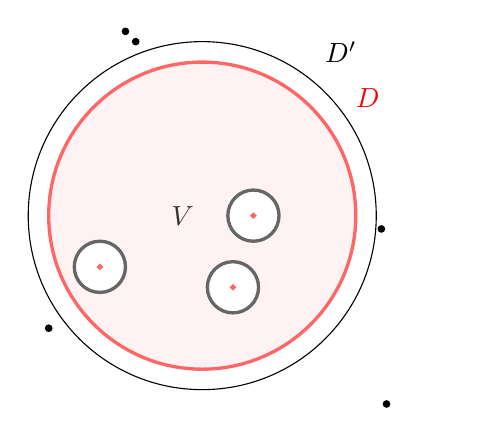
\begin{tikzpicture}[scale=1.3]
                \filldraw[color=red!60, fill=red!5, very thick](0,0) circle (1.5);
                \node[text width=1.3cm] at (1.7,1.6) {$\mathscr D'$};
                \draw[color=black](0,0) circle (1.7);
                \node[text width=1.3cm,color=red] at (2.0,1.15) {$\mathscr D$};
                \filldraw[color=black!60, fill=white, very thick](0.5,0) circle (0.25);
                \filldraw[color=red!60, fill=red!60, very thick](0.5,0) circle (0.01);
                \filldraw[color=black!60, fill=white, very thick](0.3,-0.7) circle (0.25);
                \filldraw[color=red!60, fill=red!60, very thick](0.3,-0.7) circle (0.01);
                \filldraw[color=black!60, fill=white, very thick](-1,-0.5) circle (0.25);
                \filldraw[color=red!60, fill=red!60, very thick](-1,-0.5) circle (0.01);
                \node[text width=1.3cm,color=black!80] at (0.2,0.0) {$\mathscr V$};
                \filldraw[color=black, fill=black, very thick](-1.5,-1.1) circle (0.02);
                \filldraw[color=black, fill=black, very thick](1.75,-0.13) circle (0.02);
                \filldraw[color=black, fill=black, very thick](-0.75,1.80) circle (0.02);
                \filldraw[color=black, fill=black, very thick](-0.65,1.70) circle (0.02);
                \filldraw[color=black, fill=black, very thick](1.8,-1.84) circle (0.02);
            \end{tikzpicture}
        \end{minipage}%
    }[7]

    For sufficiently small $\delta \gt 0$ the disks $\Delta _{s,\delta }$ defined by $|T -s | \le \delta $ for $s\in S$ are disjoint and contained in $\mathscr D$. Taking the affinoid $\mathscr V$ to be the complement of the union of these disks inside of $\mathscr D$.

    On the space $\mathscr V$ the series $a_i$ are approximated arbitrarily well by polynomials $b_i\in K\lb T\rb $.

    We can therefore let $g = \sum b_i W^i \in K\lb T\rb \lb W\rb $ in such a way that $C = K\lb T\rb \lb W\rb /(g)$ is a finite $K\lb T\rb $-algebra.
    Which above $\mathscr V$ is etale and isomorphic to the algebra corresponding to $\mathscr U$.

    $C$ will be ramified over the affine line over $K$ at finitely many points, so there exists some $\epsilon  \gt  0$ such that $C$ is etale over the annulus $1 \lt |T| \le 1 + \epsilon $.

    Therefore $C$ defines for us such an etale cover.

    To prove uniqueness we must first introduce some more results on models.
\end{proof}

Let $n$ be an integer $> 0$. Consider the closed rigid disk $v(T) \ge -1/n$, as the union of the unit disk $v (T) \le  0$ and the closed annulus $0 \ge v (T) \ge-1/n$. The formal model $D^{(n)}$ is no longer affine.

$D^{(n)}$ can be obtained by gluing the standard disc $\mathscr D$, with coordinate $x$, having coordinate  ring $R \{x\}$, with the annulus $C^{(n)}$ with coordinate ring $R \{x, y\} / (x^n y - \pi)$. Gluing is done on the annulus of zero thickness, which has coordinate ring $R \{x, x \inv\}$. The special fiber $D_k^{(n)}$ has two irreducible components, a projective line with multiplicity $1$ and an affine line $A_k$ with multiplicity $n$.

The two components intersect transversely at a point $\infty $.

On $P_k$ is a point called $0$ that all points with $v(T) \gt 0$ specialise to.

If $n' \gt n$ is an integer, there is a natural inclusion of disks as $v(T) \ge -1/n'$ implies $v(T) \ge -1/n$.
This induces a morphism of the formal models
\[
    D^{(n')} \to D^{(n)}
\]
when we reduce to the special fibre it identifies the $P_k$ components and sends the component $A_k$ of multiplicity $n$ to the point $\infty $.

%\InsertBoxR{0}{\begin{minipage}{0.31\linewidth}
%        \centering
\begin{figure}[H]
    \centering
        \begin{tikzpicture}[scale=1.3]
            %\node[text width=1.3cm] at (1.7,1.6) {$\mathscr D'$};
            \draw[color=black,thick](0,3) to (1,3) to (1,4);
            \draw[color=black,thick](0,0) to (1,0) to (2,1);
            \draw[color=black,thick,->](0.5,2) to (0.5,1);
            \node[text width=0.3cm] at (-0.2,0) {$0$};
            \node[text width=0.3cm] at (-0.2,3) {$0$};
            \node[text width=0.3cm] at (1.2,0) {$\infty $};
            \node[text width=0.3cm] at (1.2,3) {$\infty $};
            \node[text width=0.3cm] at (0.6,-0.2) {$P_k$};
            \node[text width=0.3cm] at (0.6,2.8) {$P_k $};
            \node[text width=0.3cm] at (1.6,0.4) {$A_k$};
            \node[text width=0.3cm] at (1.6,3.4) {$A_k $};
        \end{tikzpicture}
    \end{figure}
%    \end{minipage}%
%}[7]

Let $\mathscr Y^{(n)}$ be a rigid rigid finite covering of $\mathscr D^{(n)}$. It extended to a unique normal formal scheme $Y^{(n)}$, finite above $D^{(n)}$.

Let us consider the morphism $Y^{(n)}_k \to D^{(n)}_k$ of the special fibers, and let $Q_k$ be the  reduced inverse image of $P_k$. Then $Q_k\to  P_k$ is finite.



\begin{theorem}[3.2.6]
    Let $X$ be a normal formal $R$-curve with generic fiber $\mathscr X$ and let $x$ be a closed point of the special fiber of $X$.

    Then the set of points $z$ in $\mathscr X$ which reduce to $x $ is an open rigid connected subspace of $\mathscr X$, it is a union of a increasing set of connected quasi-compact opens.
\end{theorem}


\begin{theorem}[3.4.2]
    For $n \gg 0$ the fibre $Q_k$ is normal at all points above $\infty $.
\end{theorem}
\begin{proof}
    Consider the normalization of $Q_k$ call it $Q_k'$, the morphism $Q_k' \to Q_k$ is a blow up at points above infinity, and so we can obtain it inside of a blow up ${Y'}^{(n)} \to Y^{(n)}$ above infinity, with $Q_k'$ being the strict transform of $Q_k$.


    This blow up introduces on the special fiber of $Y$, irreducible components above the point $\infty $. Let $E$ be the open subscheme of the formal scheme ${Y'}^{(n)}$ which, on the special fiber, is the complement of the union of the irreducible components which are finite on $D_k^{(n)}$ and let $\mathscr E$ be its generic fiber. Then $E$ lies above the open annulus $0 > v(T)> - 1 / n$ and by the maximum modulus principle, there exists an integer $n' \gt n$ such that on $\mathscr E$, we have $v(T) < -1/n'$.


    So let's make the base change $D^{(n')} \to D^{(n)}$ and remove the $\pi $-torsion  from the fiber product ${Y'}^{(n)} \times_{D^{(n)}} {D^{(n')}}$. We then obtain a formal $R$-scheme $Z$ which is now finite over $D^{(n')}$ as it is disjoint from $E \times_{D^{(n)}} D^{(n')}$. Consequently, if we normalize $Z$, we find the model $Y^{(n')}$. Then, like $Y^{(n)}$ dominates $Y^{(n')}$, the closed sub-scheme of its reduced special fiber located above the component $P_k$ is still normal at infinity.
\end{proof}

We now assume $n$ is chosen such that this holds.

\begin{theorem}[3.4.6]
    For each integer $n \gt 0$ consider the formal $R$-model $D^{(n)}$ of the rigid disk $\mathscr D^{(n)}$ defined by $v(T) \ge - 1/n$.

    Write $P_k$ (resp.\ $A_k$) for the irreducible component of the projective (resp.\ affine) line of the special fibre of $D^{(n)}$ and write $\infty $ for the point of intersection of these fibres.

    Let $\mathscr U^{(n)} \to \mathscr D^{(n)}$ be a rigid finite etale cover and $U^{(n)} \to D^{(n)}$ the finite morphism of normal formal schemes which extends it.

    We write $Q_k$ for the reduced subscheme of the special fibre of $U^{(n)}$ which lies above $P_k$ and $y_i$ for $i\in I$ for the points above $\infty $. Then for $n$ sufficiently large $Q_k$ is normal above the point $\infty $.

    Letting $\mathscr U_i^{(n)}$ be the set of points $z$ of $\mathscr U^{(n)}$ that reduce to $y_i$ the map $y_i \mapsto \mathscr U_i^{(n)}$ induces a natural bijection between the points of $Q_k$ lying above infinity and the connected components of the cover $\mathscr U^{(n)} \to \mathscr D^{(n)}$ above the open annulus $0 \gt   v(T) \gt   -1/n$.

    These components remain connected when restricted to $0\gt  v(T)\gt   -1/n'$ for any $n' \gt n$.
\end{theorem}

\begin{proof}
    The normality of $Q_k$ is proved in 3.4.2.

    The points $z$ of $\mathscr U^{(n)}$ above the annulus specialise in $U_k^{(n)}$ to the points $y_i$ for $i \in I$.

    On the other hand $U^{(n)}$ is normal so by 3.2.6 the rigid open subspaces given by taking those that reduce to a single point are connected, hence they are the connected components of the cover.

    If $n'\gt  n$ the canonical morphism $U^{(n')} \to U^{(n)}$ induces the identity on $Q_k$ and is normal at infinity, hence the restriction of $\mathscr U_i^{(n)}$ to the smaller annulus remains connected.
\end{proof}


\emph{Interlude:} The complex picture. Consider the extension of function fields
\[
    \CC ( \sqrt{ x} , \sqrt{x+1}) / \CC(x)
\]
this is a $V_4$ extension with $\sqrt x \mapsto \pm \sqrt x, \sqrt{x+1} \mapsto \pm \sqrt{x+1}$.

We can take a primitive element to be $y = \sqrt x + \sqrt {x+1}$ so that
\[
    y^2 = x + x + 1 + 2\sqrt{x}\sqrt{x+1}
\]
and
\[
    (y^2 - 2x - 1)^2 - 4 x(x+1) = 0
\]
is an equation for the curve $C$ giving the cover $C \xrightarrow{x} \PP^1$.

(Ignoring infinity for this story).

This cover is ramified at the locus where $4y(y^2 - 2x - 1) = 0$, i.e.\ when $y=0$ or $\pm \sqrt{2x+1}$.
In the $y=0$ case we have 
\[(2x + 1)^2 - 4 x(x+1) = 0\]
i.e.
\[1 = 0\]
so this point does not lie on the curve.

For $y = \pm \sqrt{2x+1}$ we have $4x(x+1)=0$ so the ramification points are $x=0,-1$.
Above $x=0$ we have two points $ y = \pm 1$ each with ramification index 2.
Above $x=-1$ we have two points $ y = \pm i$ each with ramification index 2.

The cover can be visualised as follows

\begin{figure}[H]
    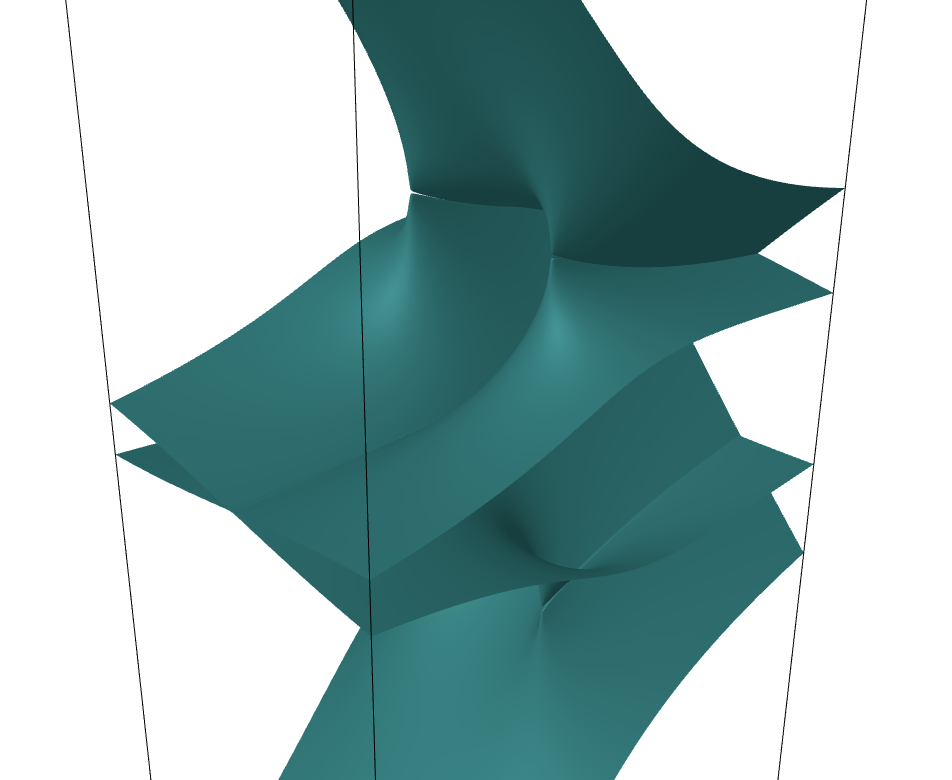
\includegraphics[width=\textwidth]{ramcov.png}
\end{figure}

Even though this looks ramified above lines instead of just points this is an artifact of the visualization.

What are the inertia groups in this case?
At $(x,y) = (0,\pm 1)$ we see that $\sqrt x$ takes on the value $0$ hence changing $\sqrt x \leftrightarrow -\sqrt x$ is in the inertia group at these points and $\sqrt{x+1}\leftrightarrow-\sqrt{x+1}$ swaps them.
At $(x,y) = (-1,\pm i)$ we see that $\sqrt {x+1}$ takes on the value $0$ hence changing $\sqrt {x+1}\leftrightarrow -\sqrt {x+1}$ is in the inertia group at these points and $\sqrt{x}\leftrightarrow-\sqrt{x}$ swaps them.






\begin{theorem}[3.4.8]
    Suppose $\mathscr U \to \mathscr D$ is a galois cover with group $G$. For $n \gg 0$ we can assume that the extended cover $\mathscr U^{(n)} \to \mathscr D^{(n)}$ is also galois with group $G$. And that the finite formal morphism $ U^{(n)} \to  D^{(n)}$ is also galois with group $G$.

    If $H_i$ is the decomposition group at the point $y_i$ then $\mathscr U^{(n)}$ is an etale galois cover of the annulus $0 \gt   v(T) \gt  -1/n$ with galois group $H_i$.

    In addition $H_i$ is a solvable group.
\end{theorem}

\begin{proof}
    For the last part. Note that if $y_i$ belongs to the irreducible component of $Q_k$, whose generic point is $\eta_i$ we can consider the decomposition group $D_i$ and the inertia group $I_i$ of $\eta_i$, and $G_i = D_i/ I_i$ acts faithfully on the component of $Q_k$, passing through $y_i$.

    Then $H_i$, is extension of the inertia subgroup of $G_i$ at $y_i$ by $I_i$.

    An inertia group of a local field is solvable, as it is an extension of a cyclic group of order coprime to the residue characteristic by a $p$ group.

\end{proof}


\end{document}
